\documentclass{article}

\usepackage[utf8]{inputenc}
\usepackage[english]{babel}

\usepackage{amsmath,amsfonts,amssymb}
\usepackage{fullpage}
\usepackage{verbatim}
\usepackage{mathabx}

\usepackage{tikz,pgfplots}

\pgfplotsset{
  width=150mm,height=100mm,
  major grid style={thin,dotted,color=black!50},
  minor grid style={thin,dotted,color=black!50},
  grid,
  every axis/.append style={
    line width=0.5pt,
    tick style={
      line cap=round,
      thin,
      major tick length=4pt,
      minor tick length=2pt,
    },
  },
  legend cell align=left,
  legend pos=north west,
}

%%%%%%%%%%%%%%%%%%%%%%%%%%%%%%%%%%%%%%%%%%%%%%%%%%%%%%%%%%%%%%%%%%%%%%%%%%%%%%%%

\begin{document}

\title{LCE-Queries}
\author{Alexander Herlez}
%\maketitle



% IMPORT-DATA stats time-2019-05-23-07-35-13.txt

\begin{center}
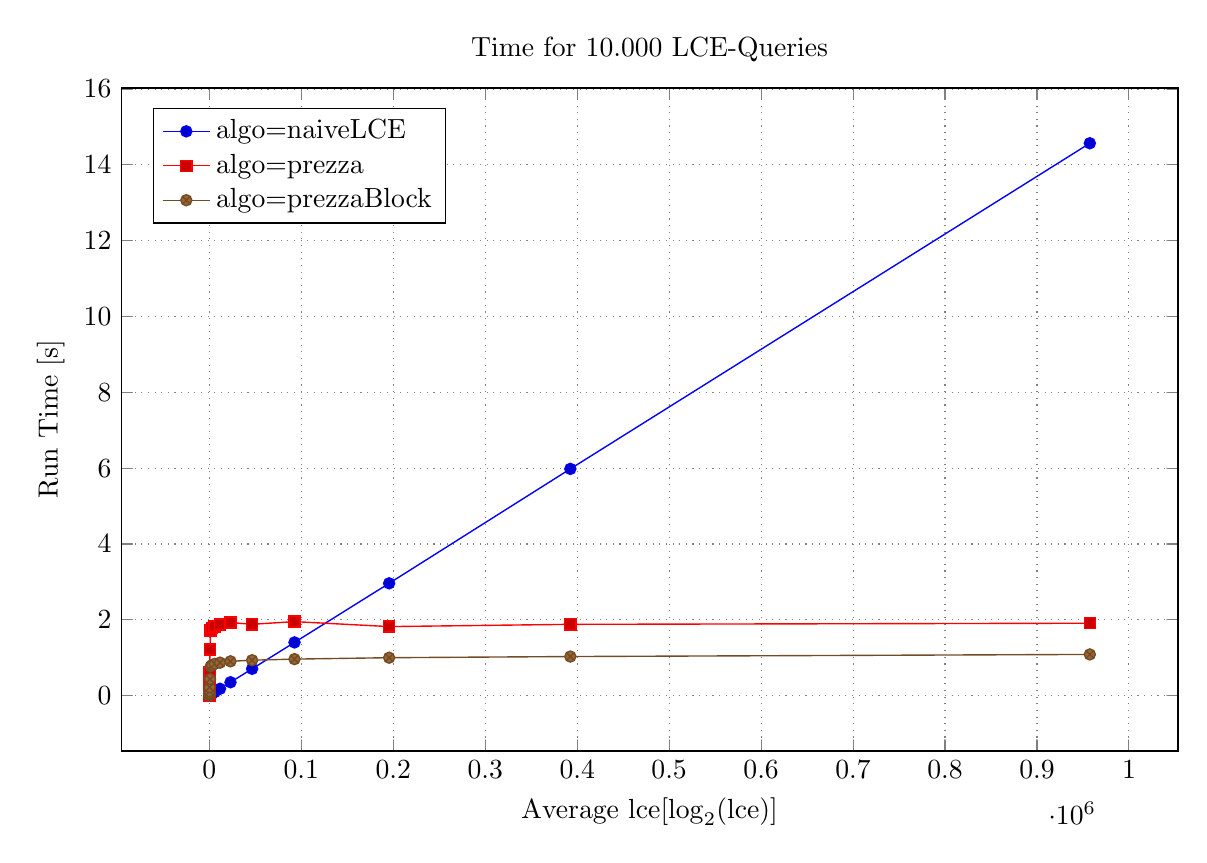
\begin{tikzpicture}
  \begin{axis}[
    title={Time for 10.000 LCE-Queries},
    xlabel={Average lce[$\log_2$(lce)]},
    ylabel={Run Time [s]},
    ]

    %% MULTIPLOT(algo) SELECT aveLCE AS x, time AS y, MULTIPLOT
    %% FROM stats GROUP BY MULTIPLOT,x  ORDER BY MULTIPLOT,x
    \addplot coordinates { (0,0.00109601) (1,0.00160503) (2,0.00244594) (6,0.0114272) (14,0.016017) (26,0.0099299) (39,0.0106881) (86,0.0143781) (174,0.017118) (360,0.0141189) (734,0.0189419) (1461,0.0297272) (2945,0.0518909) (5827,0.0952921) (11581,0.181973) (22996,0.354093) (46502,0.708684) (92591,1.40452) (195505,2.96314) (392544,5.98153) (957456,14.5695) };
    \addlegendentry{algo=naiveLCE};
    \addplot coordinates { (0,0.00536299) (1,0.00742507) (2,0.011167) (6,0.0246069) (14,0.039881) (26,0.0578279) (39,0.0816269) (86,0.165323) (174,0.313554) (360,0.610948) (734,1.21615) (1461,1.72467) (2945,1.78441) (5827,1.82072) (11581,1.87453) (22996,1.92896) (46502,1.88326) (92591,1.95319) (195505,1.8221) (392544,1.8817) (957456,1.91089) };
    \addlegendentry{algo=prezza};
    \addplot coordinates { (0,0.010006) (2,0.011699) (6,0.0194781) (14,0.025614) (26,0.029953) (39,0.0399611) (86,0.0675271) (174,0.116371) (360,0.221709) (734,0.438456) (1461,0.773158) (2945,0.806381) (5827,0.839245) (11581,0.871551) (22996,0.906404) (46502,0.935716) (92591,0.964457) (195505,1.00179) (392544,1.03239) (957456,1.08804) };
    \addlegendentry{algo=prezzaBlock};

  \end{axis}
\end{tikzpicture}
\end{center}

\end{document}
